\documentclass{article}[12pt]
\usepackage{graphicx} % Required for inserting images
\usepackage{listings}
\usepackage{hyperref}
\usepackage{tabularx}
\usepackage{float}
\usepackage{subfig}
\usepackage[a4paper, left=1cm, right=1cm]{geometry}

\title{EARIN Lab 5 Report}
\author{Krzysztof Rudnicki, 307585 \\ Jakub Kliszko, 303866  }
\date{\today}

\begin{document}

\maketitle

\section{Exercise Variant 2}
Use \href{https://pytorch.org/vision/stable/generated/torchvision.datasets.MNIST.html#torchvision.datasets.MNIST}{MIST} dataset. Evaluate at least 3 different numbers/values/types of:
\begin{itemize}
    \item learning rate
    \item mini-batch size (including batch containing only 1 example)
    \item number of hidden layers (including 0 hidden layers - linear model)
    \item width (number of neurons in hidden layers)
    \item optimizer type (e.g., SGD, SGD with momentum, Adam)
\end{itemize}

\section{Implementation}
Program can be ran by installing python, moving to project directory and issuing command:
\begin{lstlisting}[language=bash]
python main.py
\end{lstlisting}
Results will be displayed on three 2d scatter plots. \\ 
Plots Title is filled with parameters used abbreviated for space sake \\ 
Abbreviatons meaning: 
\begin{itemize} 
    \item lr - Learning Rate
    \item bs - Batch Size 
    \item hl - Number of Hidden Layers 
    \item w - Width 
    \item Adam or SGD or SGD\_Momentum - Optimizer type
\end{itemize}
Plot types: 
\begin{itemize}
    \item Loss value for learning step
    \item Train Accuracy for epoch
    \item Validation Accuracy for epoch
\end{itemize}

\begin{figure}[H]
    \caption{Exemplary plot of loss for learning Step \\ lr0.001-bs64-hl1-w128-Adam }
    \includegraphics[width=\textwidth]{testsResults/loss/def.png}
    \centering
    \end{figure}
\begin{figure}[H]
    \caption{Exemplary plot of Validation Accuracy for epoch \\ lr0.001-bs64-hl1-w128-Adam }
    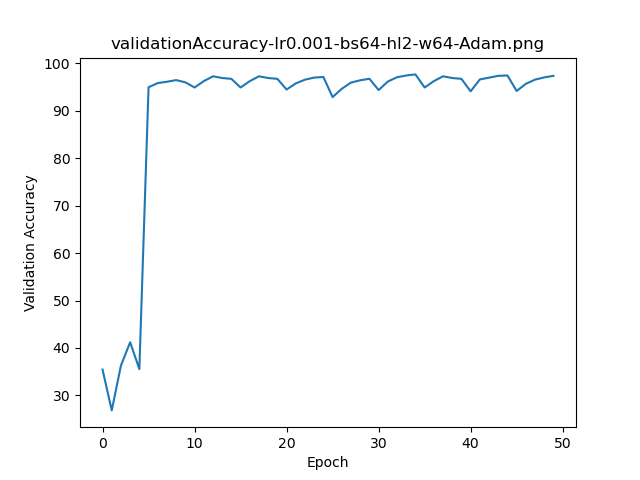
\includegraphics[width=\textwidth]{testsResults/validationAccuracy/validationAccuracy-lr0.001-bs64-hl2-w64-Adam.png}
    \centering
    \end{figure}
\begin{figure}[H]
\caption{Exemplary plot of Train Accuracy for epoch \\ lr0.001-bs64-hl1-w128-Adam }
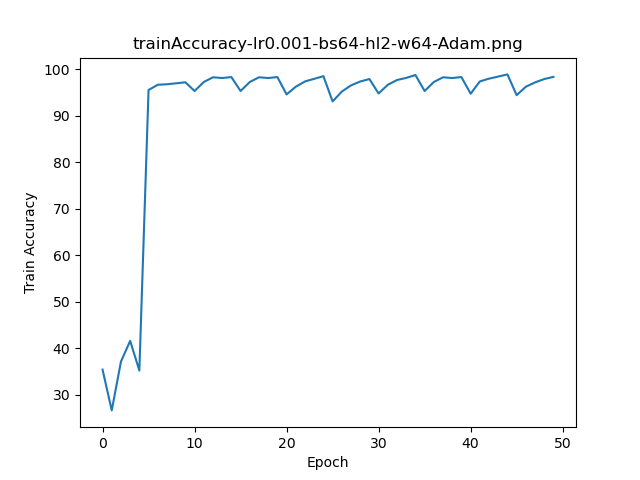
\includegraphics[width=\textwidth]{testsResults/trainAccuracy/trainAccuracy-lr0.001-bs64-hl2-w64-Adam.png}
\centering
\end{figure}
Results will be displayed and saved in the same folder as code directory for further inspection, with file name containing information about input parameters \\
Additionaly speed it took for neural network to run will be saved to results.txt along with what parameters were used \\ 
We decided to run 19 tests in total:
\begin{enumerate} 
    \item learning rate [0.1, 0.01, 0.001] (3 tests)
    \item mini-batch size [1, 64, 128, 256] (4 tests)
    \item number of hidden layers [0, 1, 2, 3] (4 tests)
    \item width [64, 128, 256, 512, 1024] (5 tests)
    \item optimizer type [SGD, SGD\_Momentum, Adam] (3 tests)
\end{enumerate} 
\section{Results}
We have successfully implemented network analyzing MNIST dataset \\ 
\subsection{Loss Graphs}

\subsubsection{Learning Rate}

    \begin{figure}[H]
        \minipage{0.5\textwidth}
        \includegraphics[width=\linewidth]{testsResults/loss/lr/def.png}
        \caption{Default settings + learning rate = 0.001}
        \endminipage\hfill
        \minipage{0.5\textwidth}
        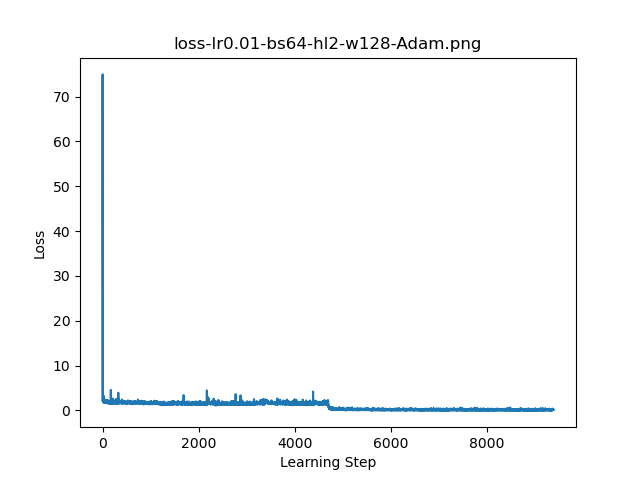
\includegraphics[width=\linewidth]{testsResults/loss/lr/loss-lr0.01-bs64-hl2-w128-Adam.png}
        \caption{Default settings + learning rate = 0.01}
        \endminipage
    \end{figure}
        \begin{figure}[H]
        \minipage{0.5\textwidth}%
        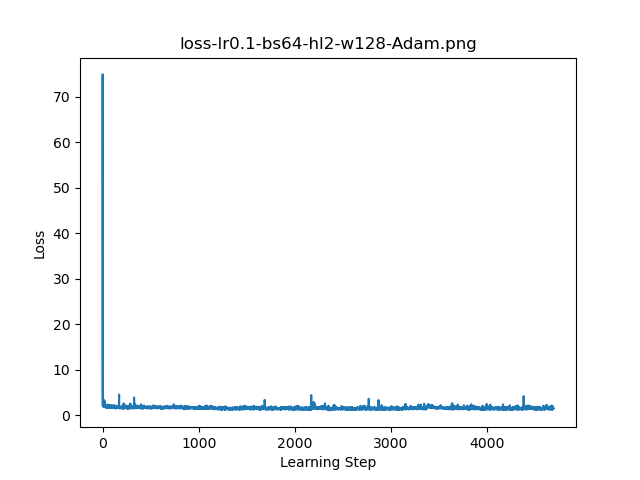
\includegraphics[width=\linewidth]{testsResults/loss/lr/loss-lr0.1-bs64-hl2-w128-Adam.png}
        \caption{Default settings + learning rate = 0.1}
        \endminipage
    \end{figure}

    \paragraph{Analysis} Smaller learning rate causes losses to drop near zero level faster (notice how there is a vertical drop for lower learning step for leaerning rate 0.001, later for learning rate 0.01 and never for learnig rate 0.1) 

\subsubsection{Mini-Batch size}

    \begin{figure}[H]
        \minipage{0.5\textwidth}
        \includegraphics[width=\linewidth]{testsResults/loss/bs/def.png}
        \caption{Default settings + batching size = 64}
        \endminipage\hfill
        \minipage{0.5\textwidth}
        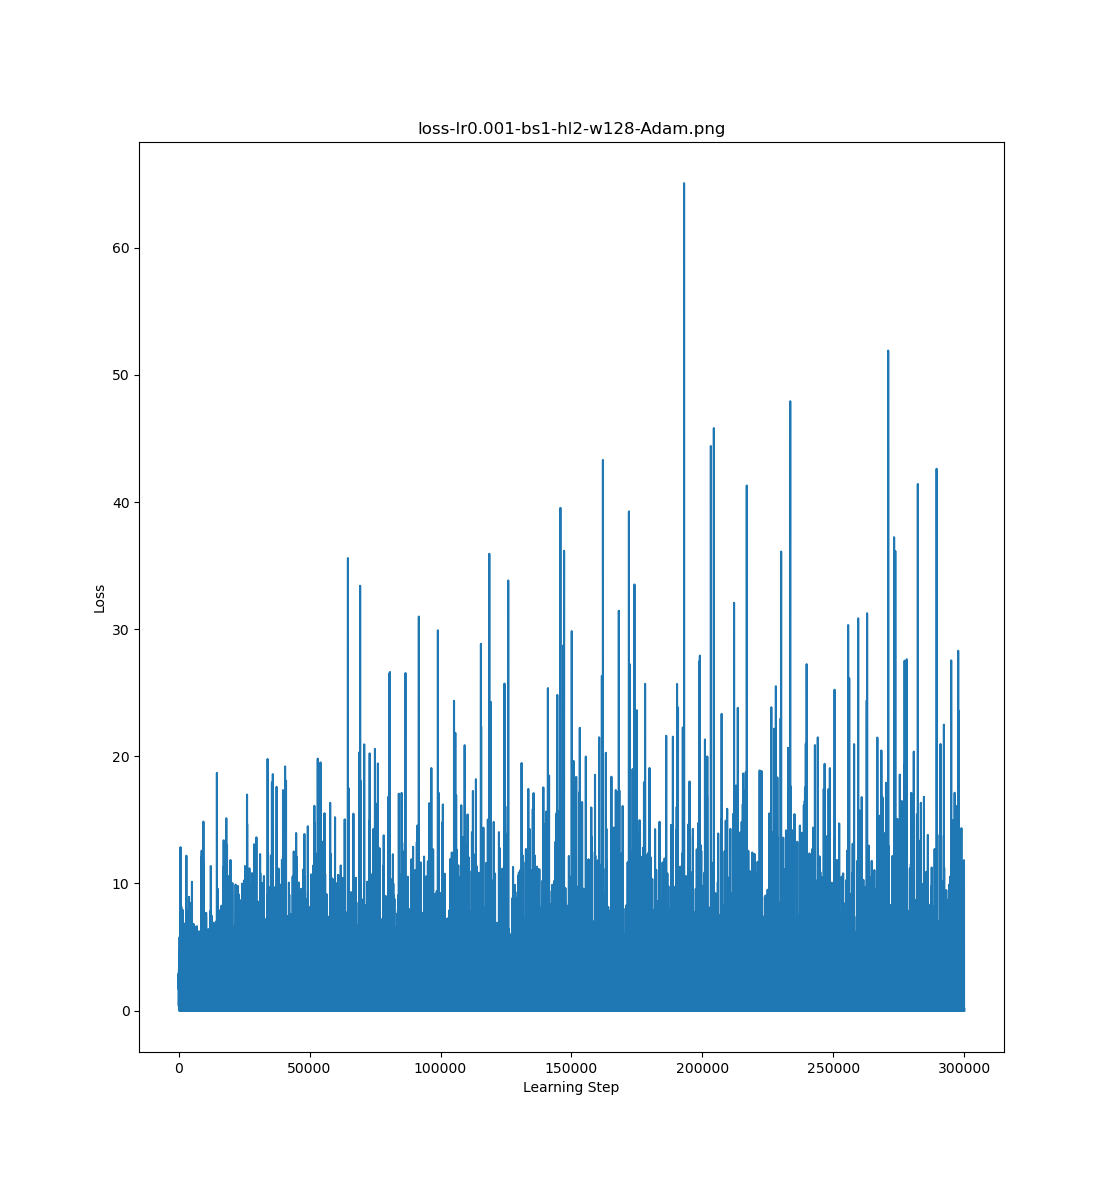
\includegraphics[width=\linewidth]{testsResults/loss/bs/loss-1batch.png}
        \caption{Default settings + batching size = 1}
        \endminipage
    \end{figure}
        \begin{figure}[H]
        \minipage{0.5\textwidth}%
        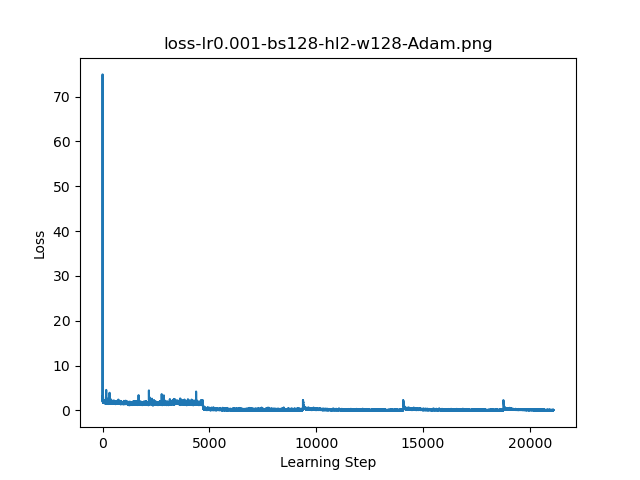
\includegraphics[width=\linewidth]{testsResults/loss/bs/loss-lr0.001-bs128-hl2-w128-Adam.png}
        \caption{Default settings + batching size = 128}
        \endminipage
        \minipage{0.5\textwidth}%
        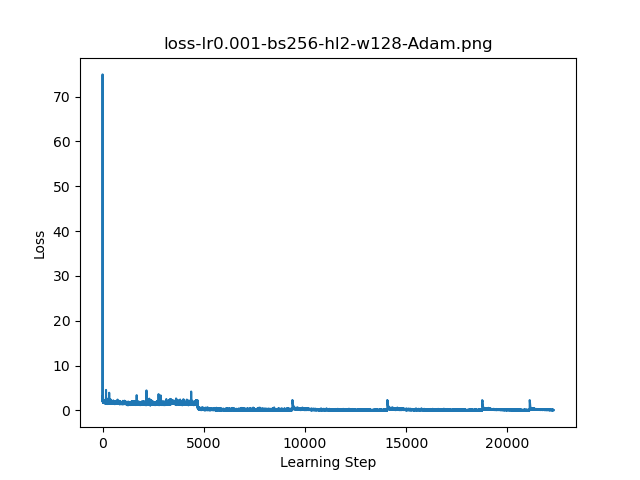
\includegraphics[width=\linewidth]{testsResults/loss/bs/loss-lr0.001-bs256-hl2-w128-Adam.png}
        \caption{Default settings + batching size = 256}
        \endminipage
    \end{figure}

    \paragraph{Analysis} Batching size equal to 1 makes losses seem pretty much random, increasing batch sizes increases 'flat' (smaller) loss periods between local peaks

\subsubsection{Number of Hidden Layers}

    \begin{figure}[H]
        \minipage{0.5\textwidth}
        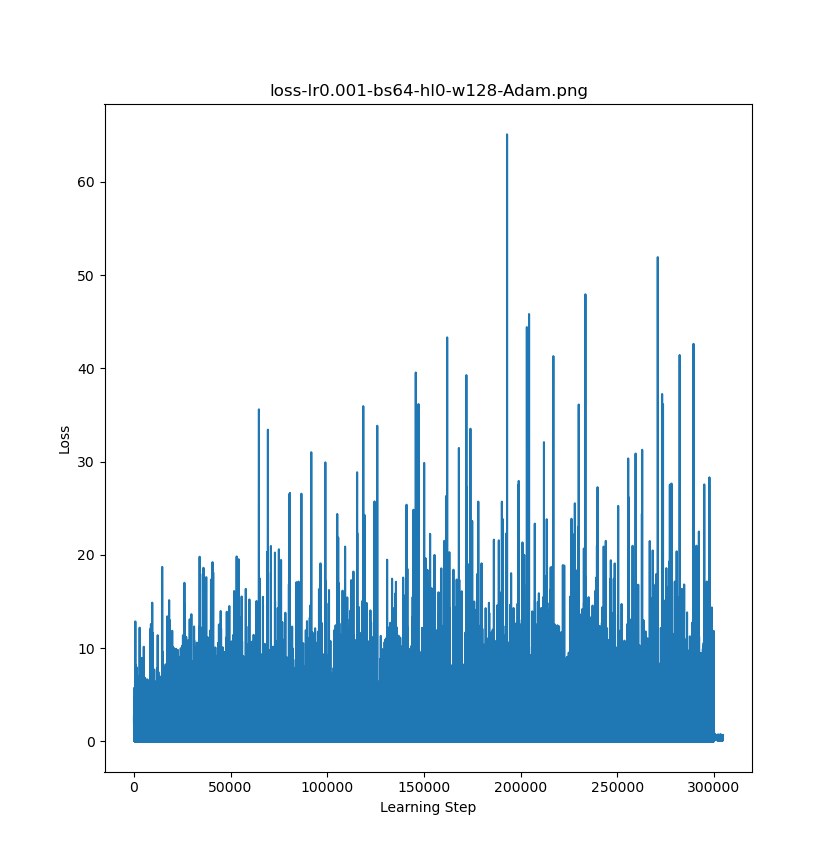
\includegraphics[width=\linewidth]{testsResults/loss/hl/hl0loss.png}
        \caption{Default settings + hidden layers = 0}
        \endminipage\hfill
        \minipage{0.5\textwidth}
        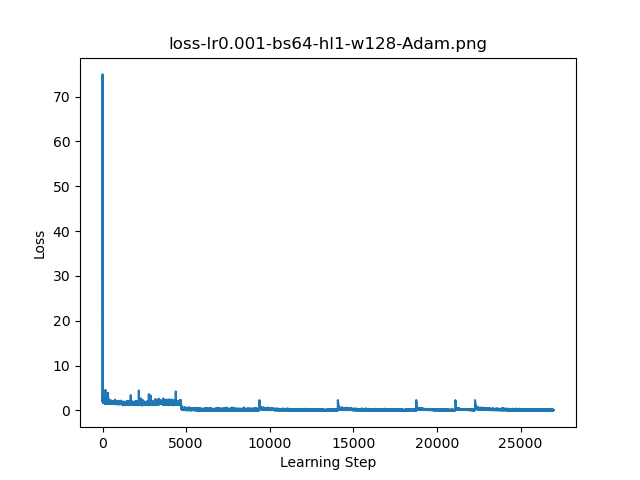
\includegraphics[width=\linewidth]{testsResults/loss/hl/loss-lr0.001-bs64-hl1-w128-Adam.png}
        \caption{Default settings + hidden layers = 1}
        \endminipage
    \end{figure}
        \begin{figure}[H]
        \minipage{0.5\textwidth}%
        \includegraphics[width=\linewidth]{testsResults/loss/hl/def.png}
        \caption{Default settings + hidden layers = 2}
        \endminipage
        \minipage{0.5\textwidth}%
        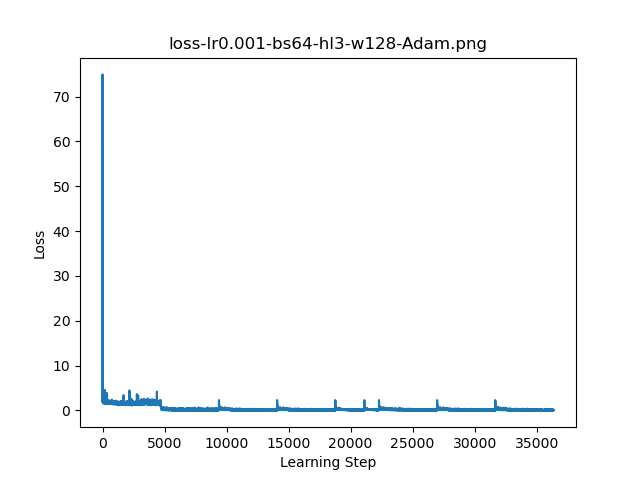
\includegraphics[width=\linewidth]{testsResults/loss/hl/loss-lr0.001-bs64-hl3-w128-Adam.png}
        \caption{Default settings + hidden layers = 3}
        \endminipage
    \end{figure}

    \paragraph{Analysis} Setting hidden layers to 0 again makes losses value seem random, hidden layer set to 1 provides us with later drop but longer flat periods, number of hidden layers set to 2 offeres the opposite and number of layers set to 3 seems to be a compromise between those two 
\subsubsection{Width}

    \begin{figure}[H]
        \minipage{0.5\textwidth}
        \includegraphics[width=\linewidth]{testsResults/loss/w/def.png}
        \caption{Default settings + width = 128}
        \endminipage\hfill
        \minipage{0.5\textwidth}
        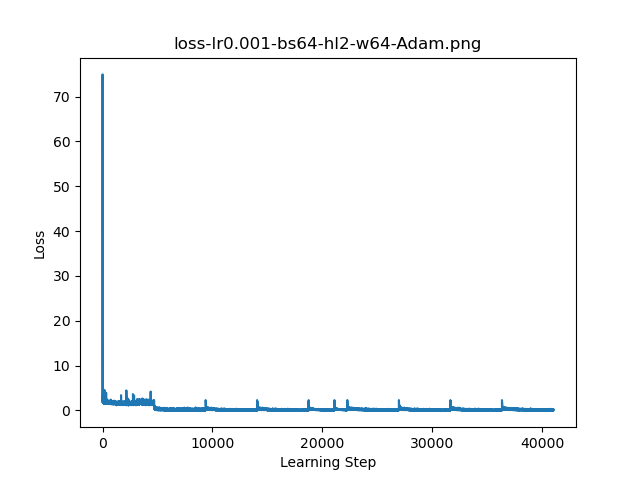
\includegraphics[width=\linewidth]{testsResults/loss/w/loss-lr0.001-bs64-hl2-w64-Adam.png}
        \caption{Default settings + width = 64}
        \endminipage
    \end{figure}
        \begin{figure}[H]
        \minipage{0.5\textwidth}%
        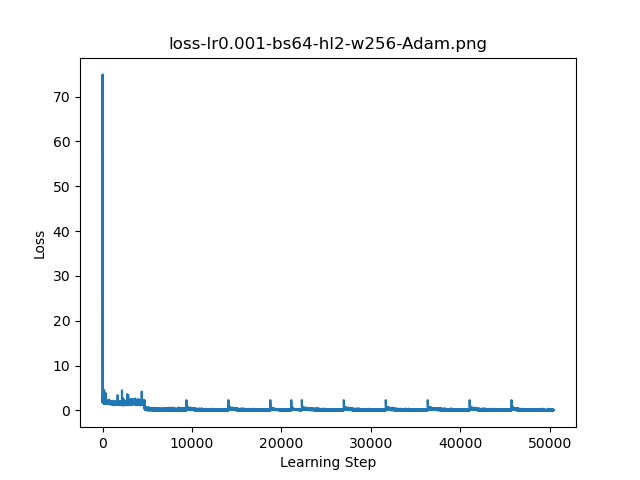
\includegraphics[width=\linewidth]{testsResults/loss/w/loss-lr0.001-bs64-hl2-w256-Adam.png}
        \caption{Default settings + width = 256}
        \endminipage
        \minipage{0.5\textwidth}%
        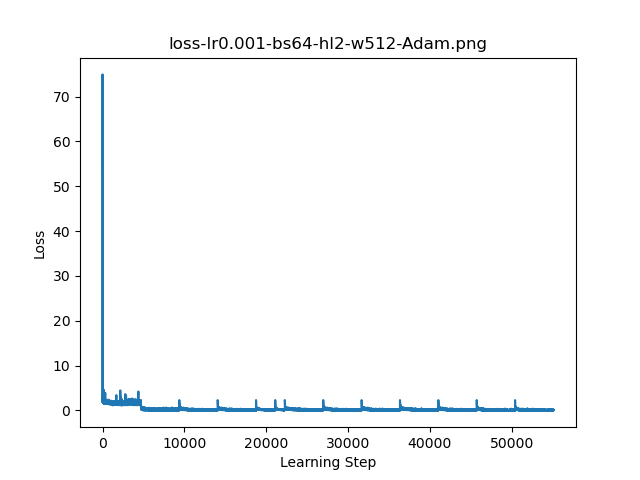
\includegraphics[width=\linewidth]{testsResults/loss/w/loss-lr0.001-bs64-hl2-w512-Adam.png}
        \caption{Default settings + width = 512}
        \endminipage
    \end{figure}
    \begin{figure}[H]
        \minipage{0.5\textwidth}%
        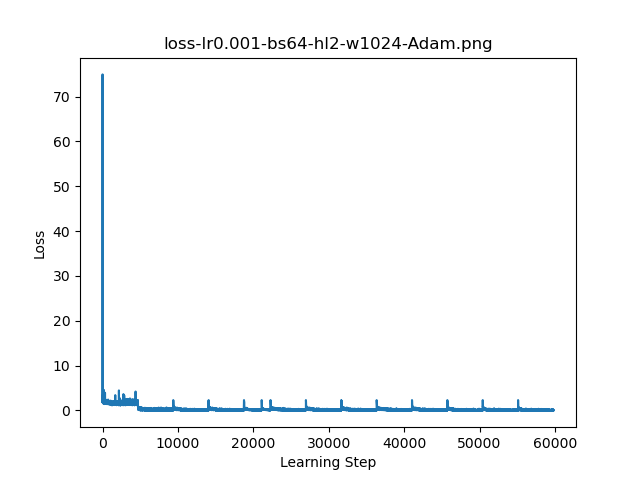
\includegraphics[width=\linewidth]{testsResults/loss/w/loss-lr0.001-bs64-hl2-w1024-Adam.png}
        \caption{Default settings + width = 1024}
        \endminipage
    \end{figure}

    \paragraph{Analysis} Changing width does not seem to affect loss greatly


\subsubsection{Optimizer Type}

    \begin{figure}[H]
        \minipage{0.5\textwidth}
        \includegraphics[width=\linewidth]{testsResults/loss/optimizer/def.png}
        \caption{Default settings + Adam optimizer}
        \endminipage\hfill
        \minipage{0.5\textwidth}
        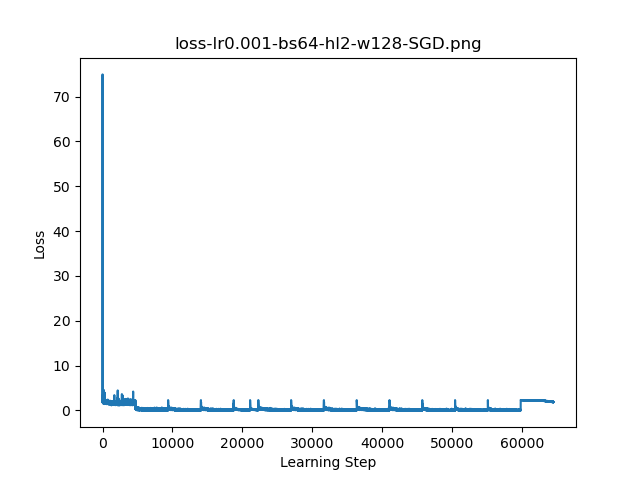
\includegraphics[width=\linewidth]{testsResults/loss/optimizer/loss-lr0.001-bs64-hl2-w128-SGD.png}
        \caption{Default settings + learning rate = 0.01}
        \endminipage
    \end{figure}
        \begin{figure}[H]
        \minipage{0.5\textwidth}%
        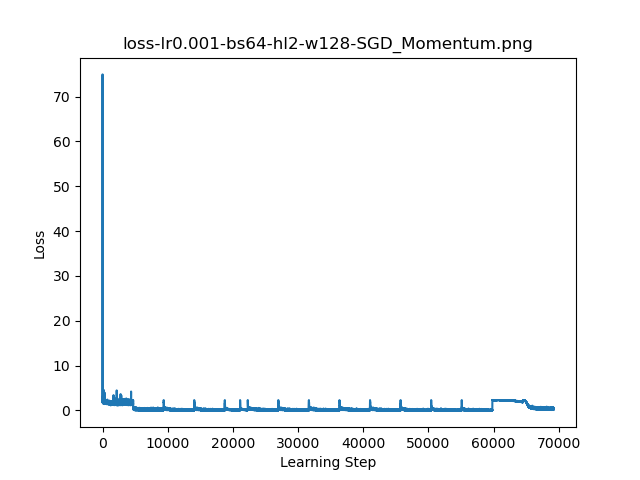
\includegraphics[width=\linewidth]{testsResults/loss/optimizer/loss-lr0.001-bs64-hl2-w128-SGD_Momentum.png}
        \caption{Default settings + SGD\_Momentum optimizer}
        \endminipage
    \end{figure}

    \paragraph{Analysis} Changing optimizers does not seem to affect loss greatly


\subsection{Train Accuracy Graphs}

\subsubsection{Learning Rate}

    \begin{figure}[H]
        \minipage{0.5\textwidth}
        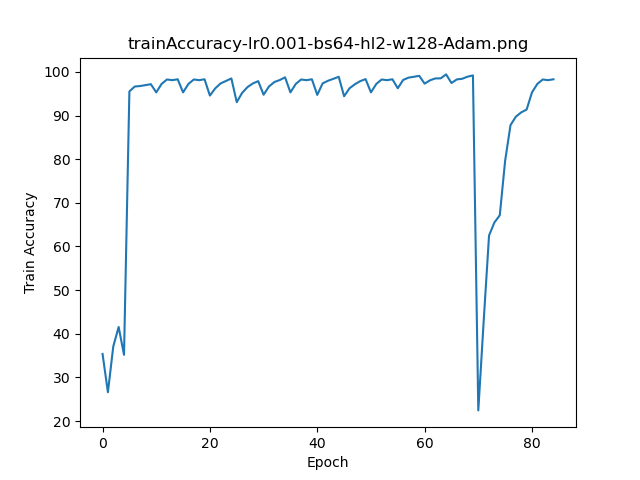
\includegraphics[width=\linewidth]{testsResults/trainAccuracy/def.png}
        \caption{Default settings + learning rate = 0.001}
        \endminipage\hfill
        \minipage{0.5\textwidth}
        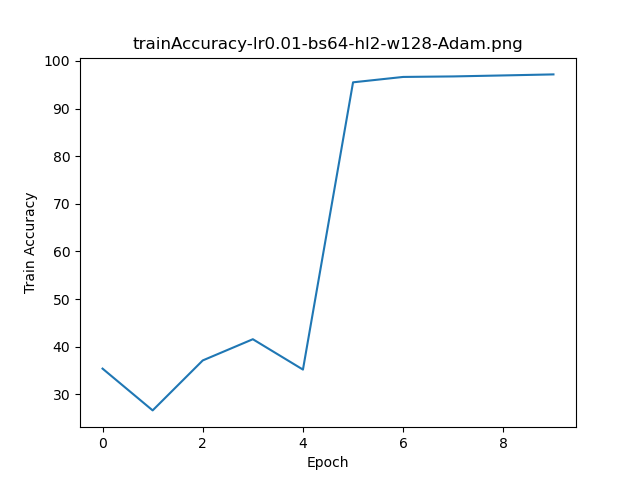
\includegraphics[width=\linewidth]{testsResults/trainAccuracy/trainAccuracy-lr0.01-bs64-hl2-w128-Adam.png}
        \caption{Default settings + learning rate = 0.01}
        \endminipage
    \end{figure}
        \begin{figure}[H]
        \minipage{0.5\textwidth}%
        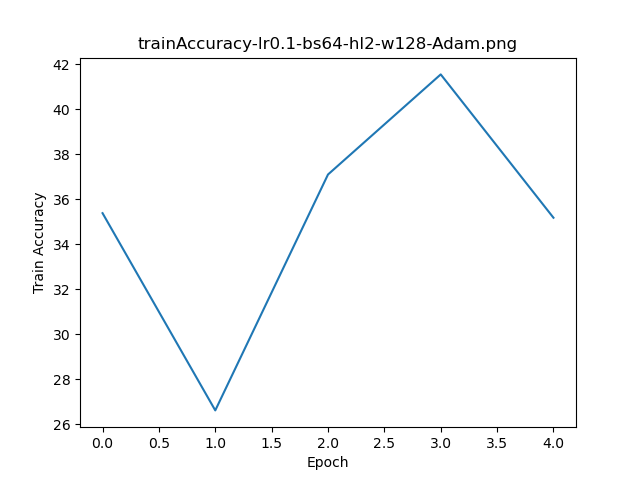
\includegraphics[width=\linewidth]{testsResults/trainAccuracy/trainAccuracy-lr0.1-bs64-hl2-w128-Adam.png}
        \caption{Default settings + learning rate = 0.1}
        \endminipage
    \end{figure}

    \paragraph{Analysis} Making training accuracy smaller than 0.01 seems to be unnecessary for this dataset as it offers little to no improve in accuracy. Setting it to 0.1 on the other hand provides very low accuracy of neural network

\subsubsection{Mini-Batch size}

    \begin{figure}[H]
        \minipage{0.5\textwidth}
        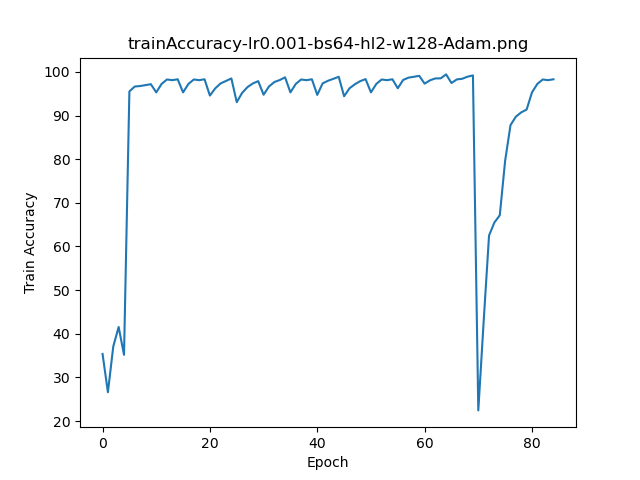
\includegraphics[width=\linewidth]{testsResults/trainAccuracy/def.png}
        \caption{Default settings + batching size = 64}
        \endminipage\hfill
        \minipage{0.5\textwidth}
        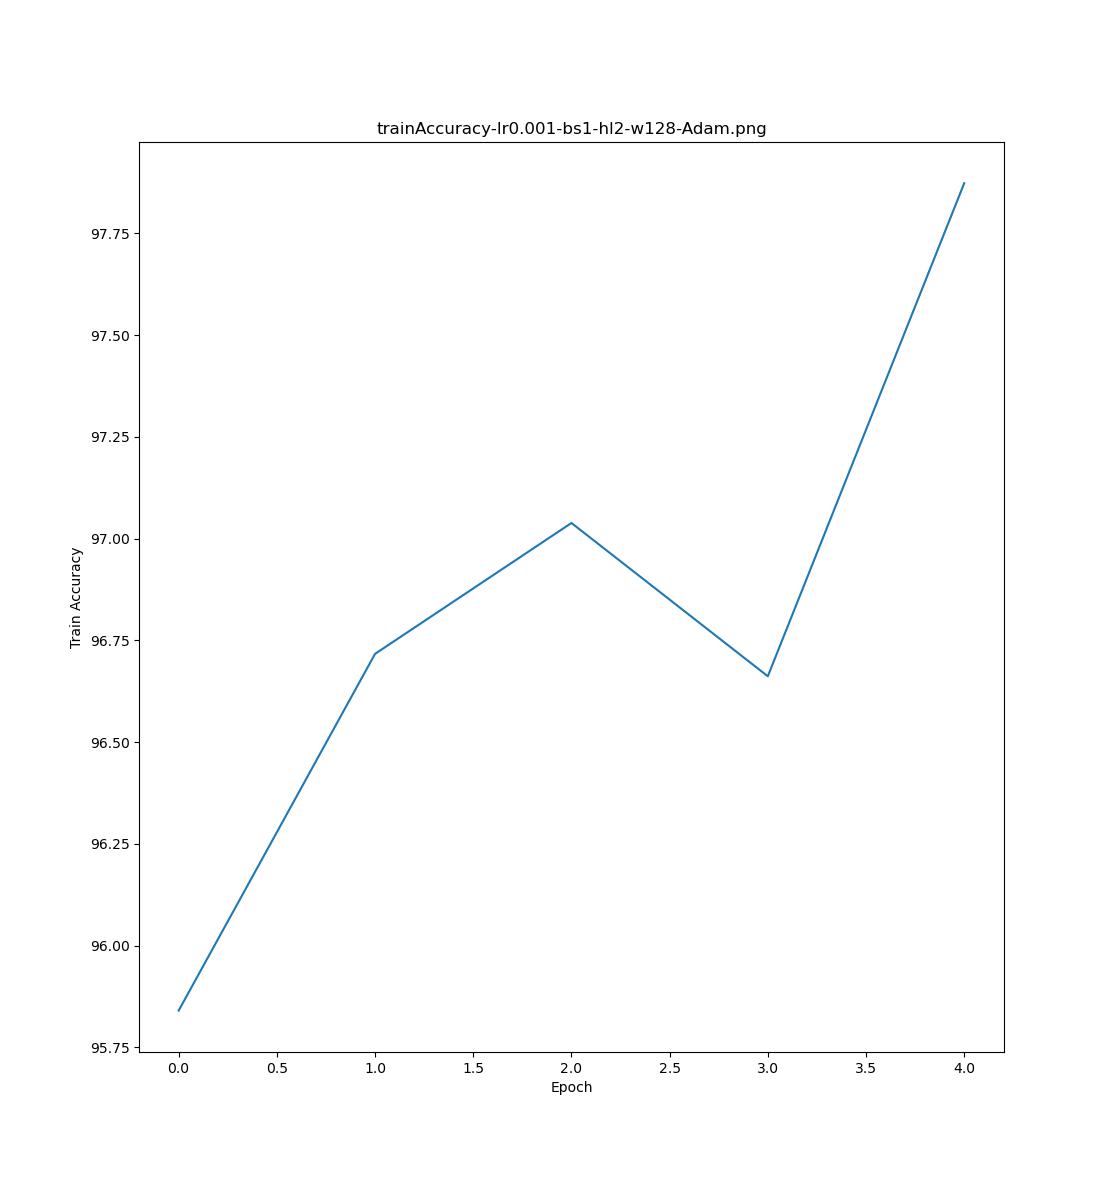
\includegraphics[width=\linewidth]{testsResults/trainAccuracy/trainAccuracy1batch.png}
        \caption{Default settings + batching size = 1}
        \endminipage
    \end{figure}
        \begin{figure}[H]
        \minipage{0.5\textwidth}%
        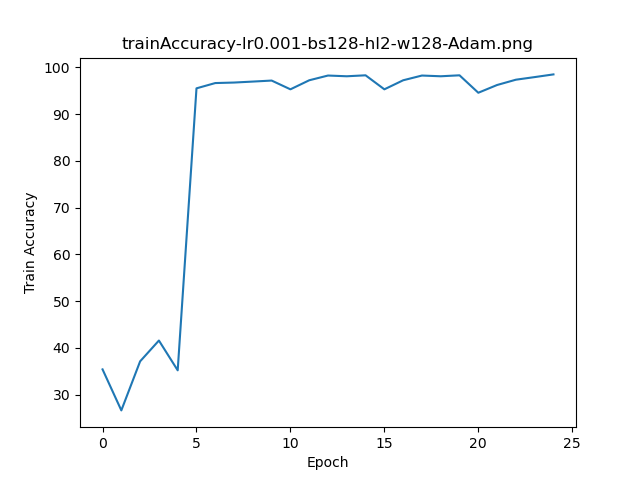
\includegraphics[width=\linewidth]{testsResults/trainAccuracy/trainAccuracy-lr0.001-bs128-hl2-w128-Adam.png}
        \caption{Default settings + batching size = 128}
        \endminipage
        \minipage{0.5\textwidth}%
        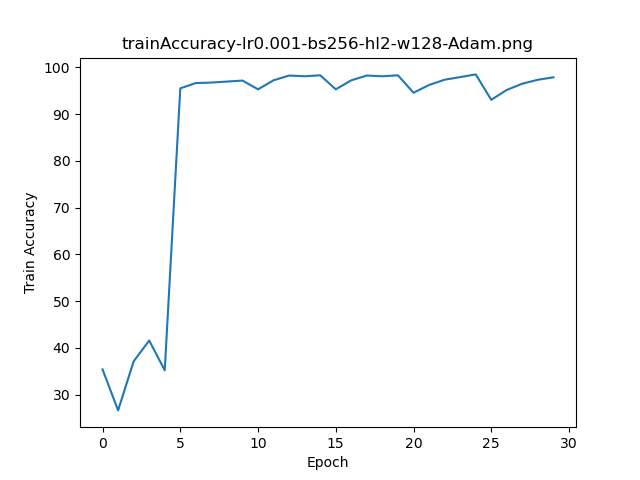
\includegraphics[width=\linewidth]{testsResults/trainAccuracy/trainAccuracy-lr0.001-bs256-hl2-w128-Adam.png}
        \caption{Default settings + batching size = 256}
        \endminipage
    \end{figure}

    \paragraph{Analysis} Increasing batching size does not seem to make drastic change for train accuracy, even setting batching size to 1 offers very good (over 95 \%) accuracy




\subsubsection{Number of Hidden Layers}

    \begin{figure}[H]
        \minipage{0.5\textwidth}
        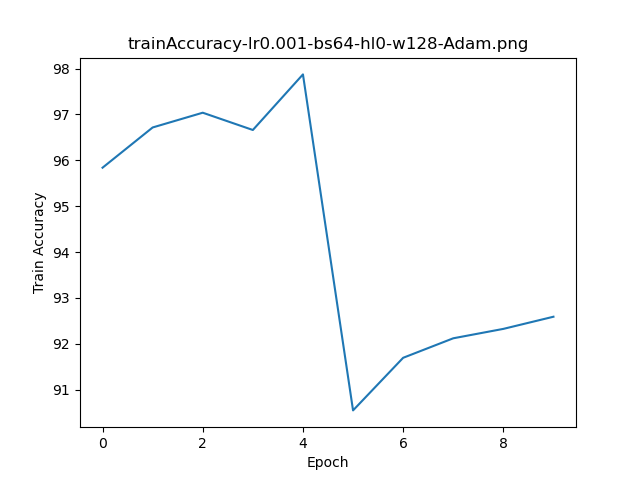
\includegraphics[width=\linewidth]{testsResults/trainAccuracy/trainAccuracy-lr0.001-bs64-hl0-w128-Adam.png}
        \caption{Default settings + hidden layers = 0}
        \endminipage\hfill
        \minipage{0.5\textwidth}
        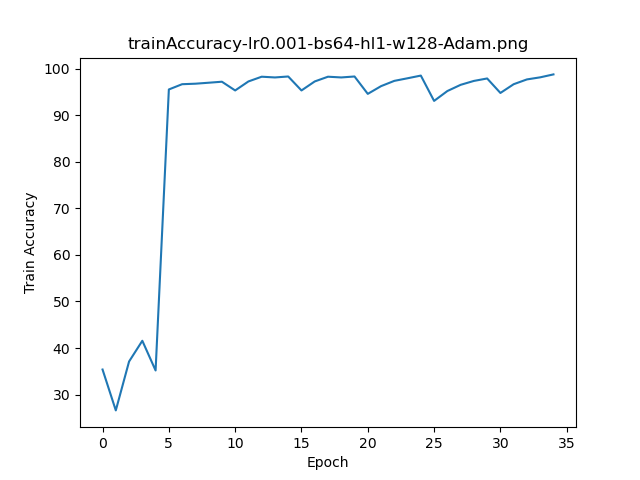
\includegraphics[width=\linewidth]{testsResults/trainAccuracy/trainAccuracy-lr0.001-bs64-hl1-w128-Adam.png}
        \caption{Default settings + hidden layers = 1}
        \endminipage
    \end{figure}
        \begin{figure}[H]
        \minipage{0.5\textwidth}%
        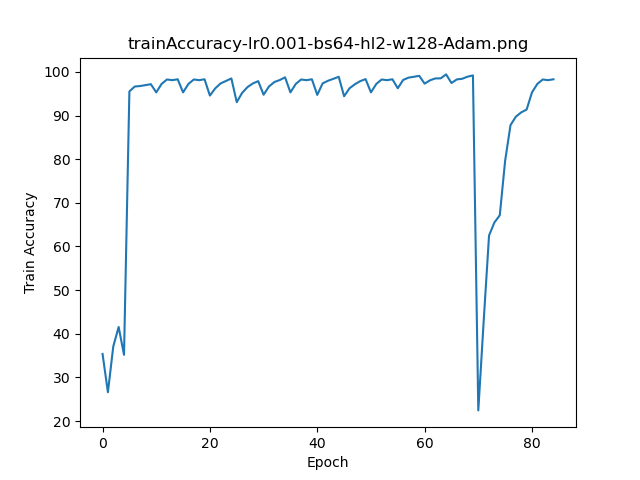
\includegraphics[width=\linewidth]{testsResults/trainAccuracy/def.png}
        \caption{Default settings + hidden layers = 2}
        \endminipage
        \minipage{0.5\textwidth}%
        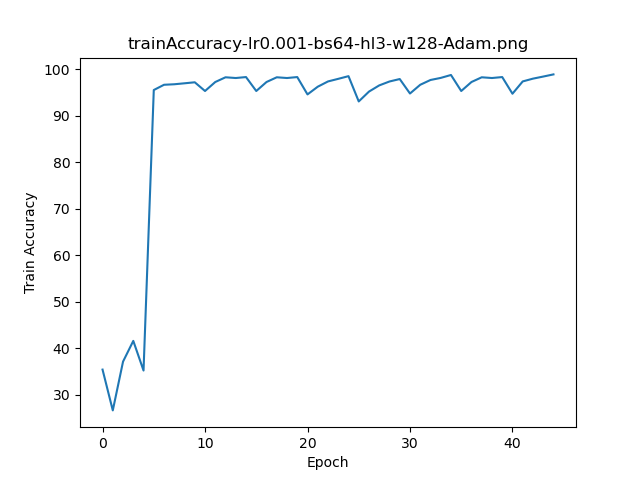
\includegraphics[width=\linewidth]{testsResults/trainAccuracy/trainAccuracy-lr0.001-bs64-hl3-w128-Adam.png}
        \caption{Default settings + hidden layers = 3}
        \endminipage
    \end{figure}

    \paragraph{Analysis} Increasing hidden layers number reduces variety of train accuracy results, with hidden layers set to 0 having accuracy vary between 91 and 98 and with hidden layers equal to 3 showing much smoother graph
\subsubsection{Width}

    \begin{figure}[H]
        \minipage{0.5\textwidth}
        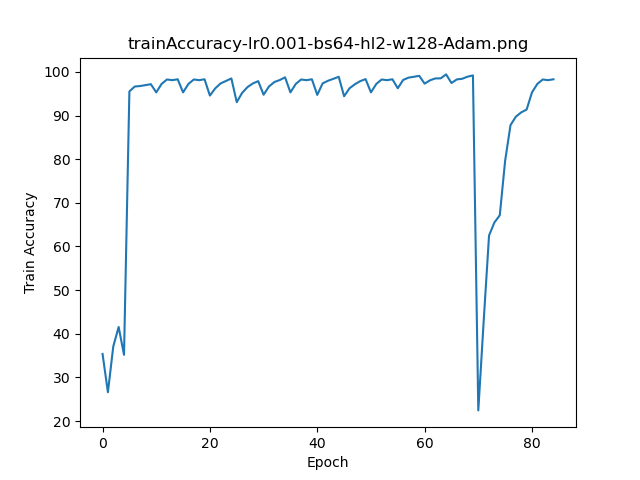
\includegraphics[width=\linewidth]{testsResults/trainAccuracy/def.png}
        \caption{Default settings + width = 128}
        \endminipage\hfill
        \minipage{0.5\textwidth}
        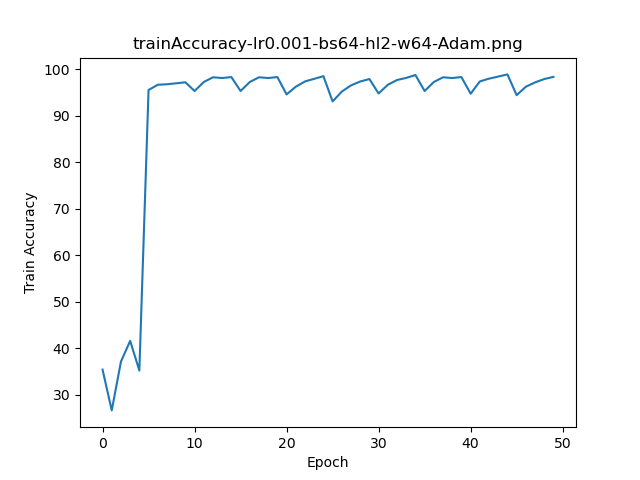
\includegraphics[width=\linewidth]{testsResults/trainAccuracy/trainAccuracy-lr0.001-bs64-hl2-w64-Adam.png}
        \caption{Default settings + width = 64}
        \endminipage
    \end{figure}
        \begin{figure}[H]
        \minipage{0.5\textwidth}%
        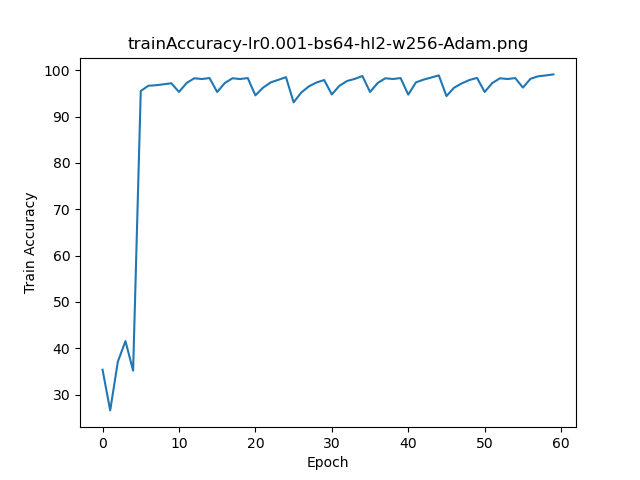
\includegraphics[width=\linewidth]{testsResults/trainAccuracy/trainAccuracy-lr0.001-bs64-hl2-w256-Adam.png}
        \caption{Default settings + width = 256}
        \endminipage
        \minipage{0.5\textwidth}%
        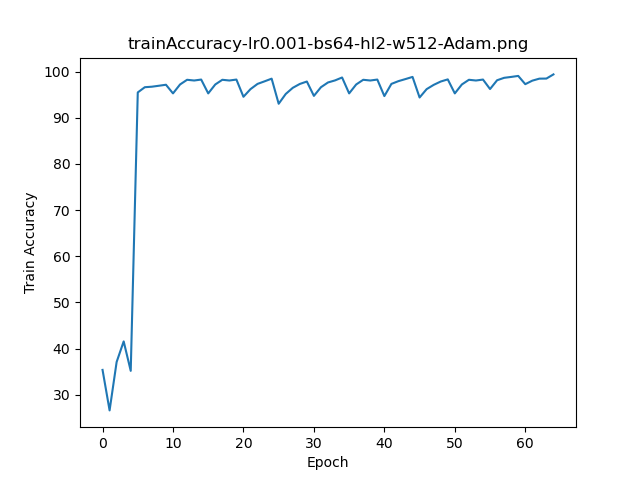
\includegraphics[width=\linewidth]{testsResults/trainAccuracy/trainAccuracy-lr0.001-bs64-hl2-w512-Adam.png}
        \caption{Default settings + width = 512}
        \endminipage
    \end{figure}
    \begin{figure}[H]
        \minipage{0.5\textwidth}%
        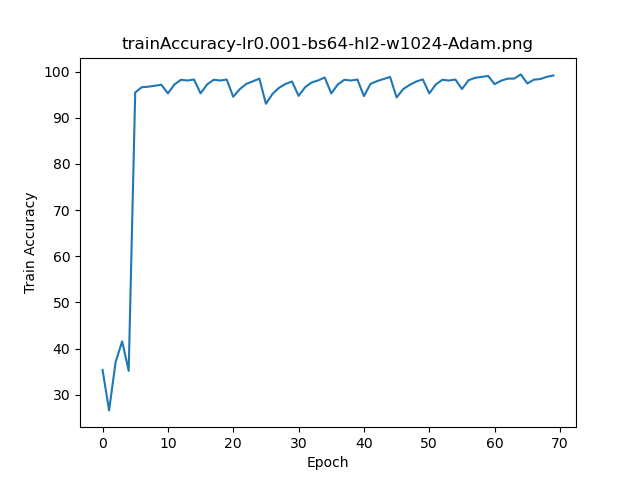
\includegraphics[width=\linewidth]{testsResults/trainAccuracy/trainAccuracy-lr0.001-bs64-hl2-w1024-Adam.png}
        \caption{Default settings + width = 1024}
        \endminipage
    \end{figure}

    \paragraph{Analysis} Changing width does not seem to influence accuracy much

\subsubsection{Optimizer Type}

    \begin{figure}[H]
        \minipage{0.5\textwidth}
        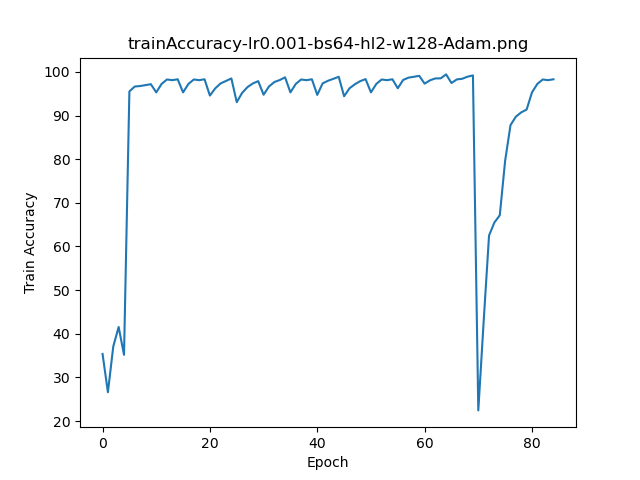
\includegraphics[width=\linewidth]{testsResults/trainAccuracy/def.png}
        \caption{Default settings + Adam optimizer}
        \endminipage\hfill
        \minipage{0.5\textwidth}
        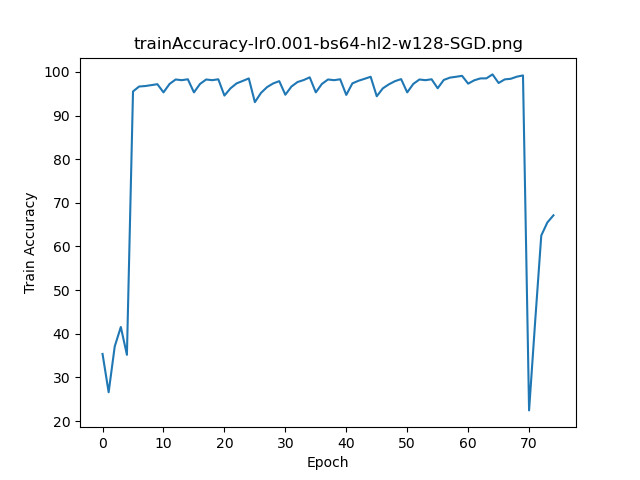
\includegraphics[width=\linewidth]{testsResults/trainAccuracy/trainAccuracy-lr0.001-bs64-hl2-w128-SGD.png}
        \caption{Default settings + learning rate = 0.01}
        \endminipage
    \end{figure}
        \begin{figure}[H]
        \minipage{0.5\textwidth}%
        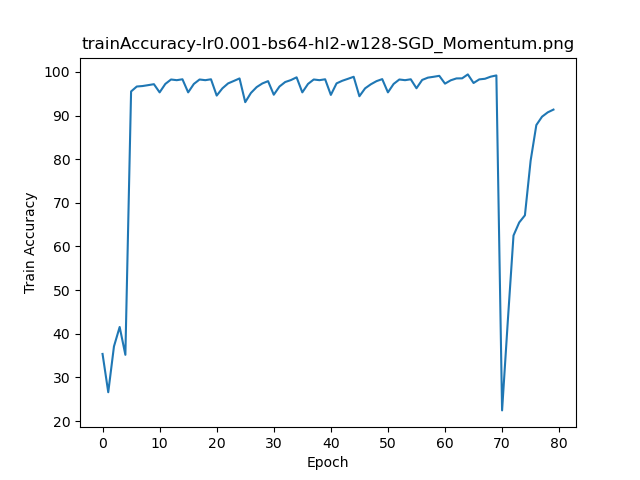
\includegraphics[width=\linewidth]{testsResults/trainAccuracy/trainAccuracy-lr0.001-bs64-hl2-w128-SGD_Momentum.png}
        \caption{Default settings + SGD\_Momentum optimizer}
        \endminipage
    \end{figure}

    \paragraph{Analysis} Changing optimizer type does not seem to influence accuracy much

\subsection{Validation Accuracy Graphs}
Validation Accuracy Graphs look similar to Train accuracy so in order not to repeat ourselves we ommited analysis of them


\subsubsection{Learning Rate}

    \begin{figure}[H]
        \minipage{0.5\textwidth}
        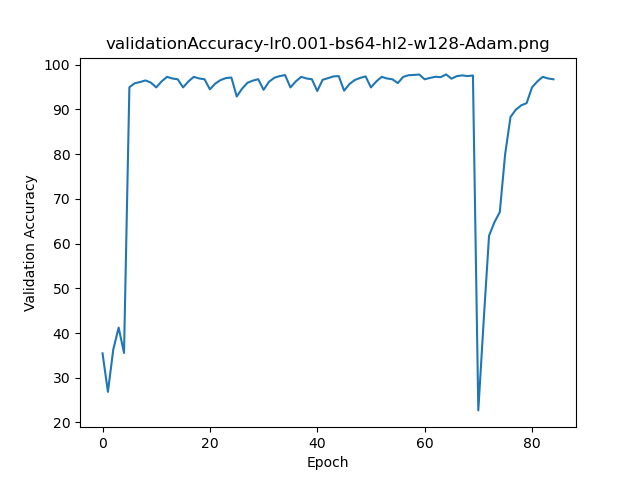
\includegraphics[width=\linewidth]{testsResults/validationAccuracy/def.png}
        \caption{Default settings + learning rate = 0.001}
        \endminipage\hfill
        \minipage{0.5\textwidth}
        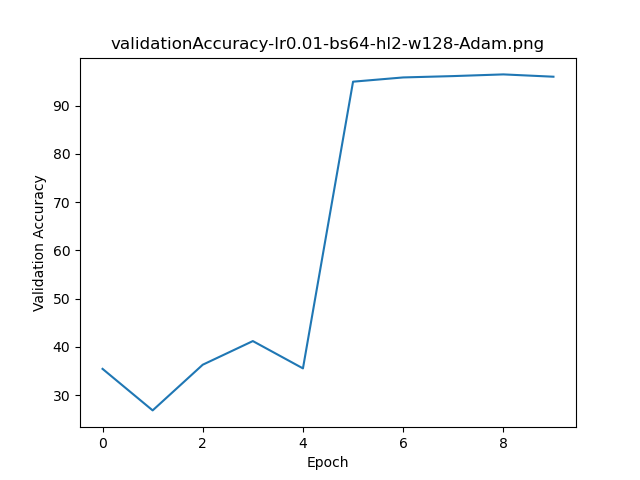
\includegraphics[width=\linewidth]{testsResults/validationAccuracy/validationAccuracy-lr0.01-bs64-hl2-w128-Adam.png}
        \caption{Default settings + learning rate = 0.01}
        \endminipage
    \end{figure}
        \begin{figure}[H]
        \minipage{0.5\textwidth}%
        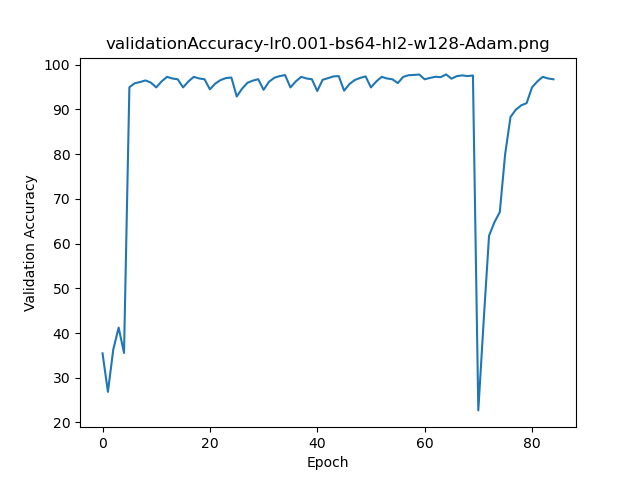
\includegraphics[width=\linewidth]{testsResults/validationAccuracy/def.png}
        \caption{Default settings + learning rate = 0.1}
        \endminipage
    \end{figure}

\subsubsection{Mini-Batch size}

    \begin{figure}[H]
        \minipage{0.5\textwidth}
        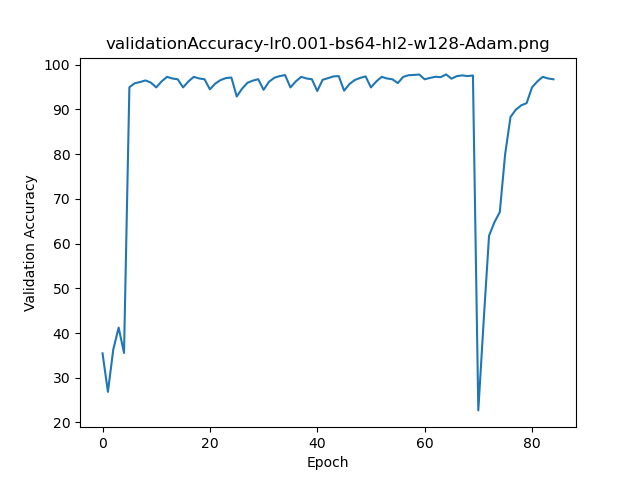
\includegraphics[width=\linewidth]{testsResults/validationAccuracy/def.png}
        \caption{Default settings + batching size = 64}
        \endminipage\hfill
        \minipage{0.5\textwidth}
        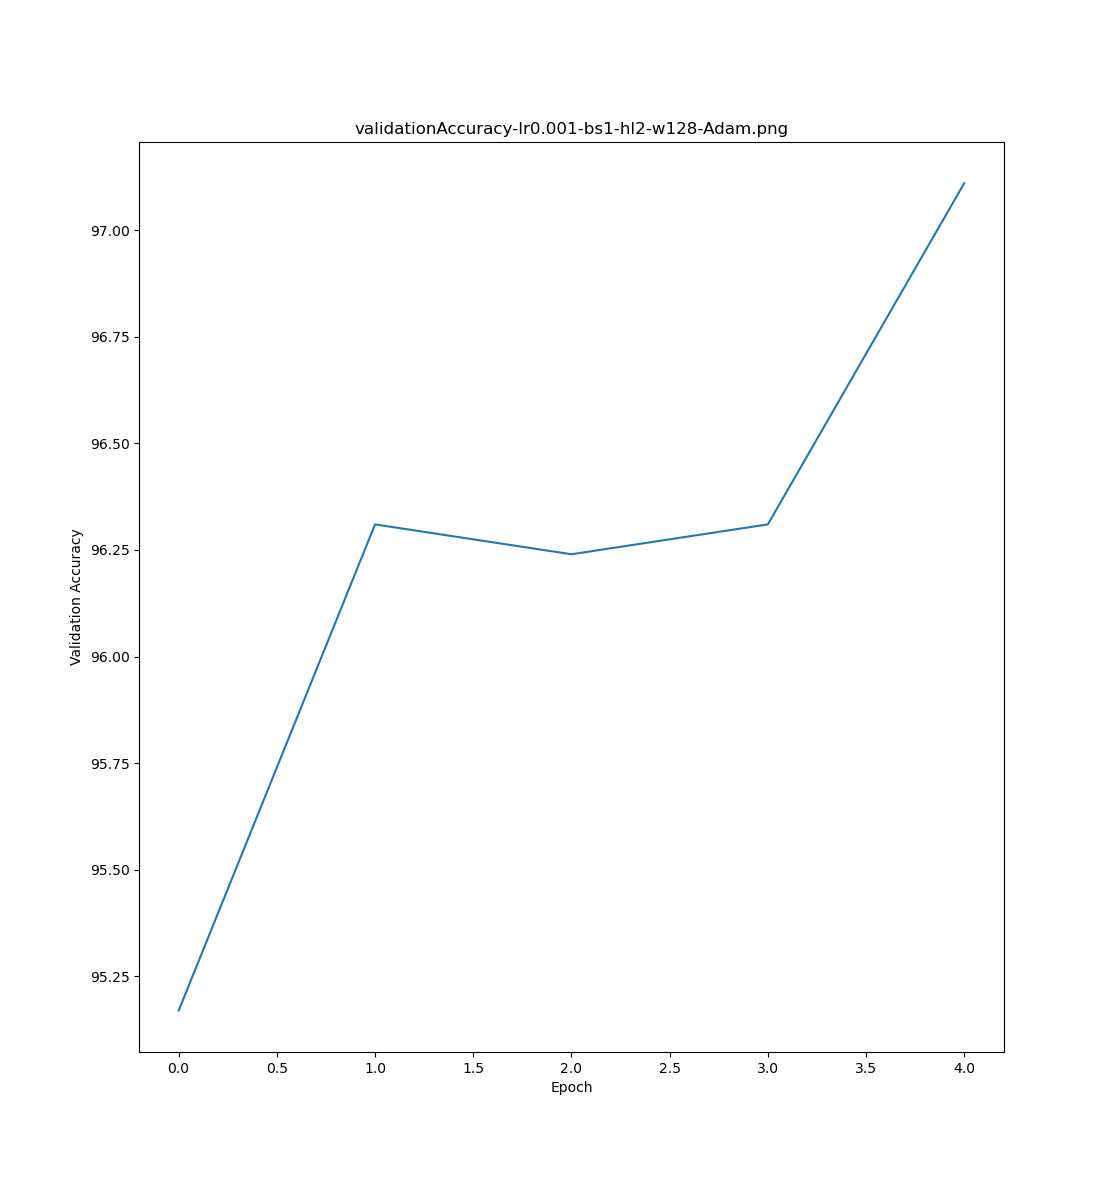
\includegraphics[width=\linewidth]{testsResults/validationAccuracy/validationAccuracy1batch.png}
        \caption{Default settings + batching size = 1}
        \endminipage
    \end{figure}
        \begin{figure}[H]
        \minipage{0.5\textwidth}%
        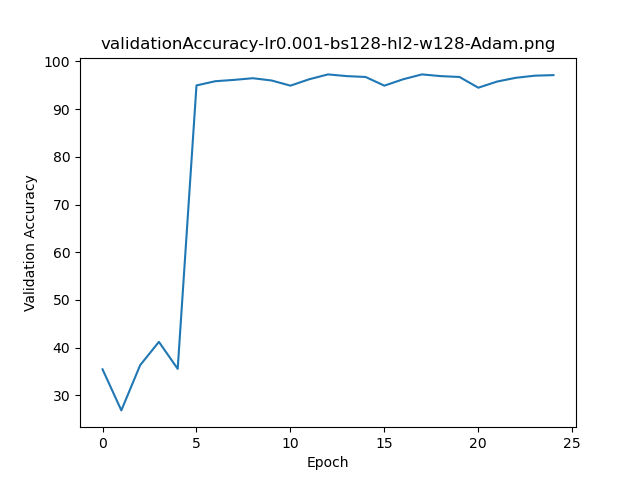
\includegraphics[width=\linewidth]{testsResults/validationAccuracy/validationAccuracy-lr0.001-bs128-hl2-w128-Adam.png}
        \caption{Default settings + batching size = 128}
        \endminipage
        \minipage{0.5\textwidth}%
        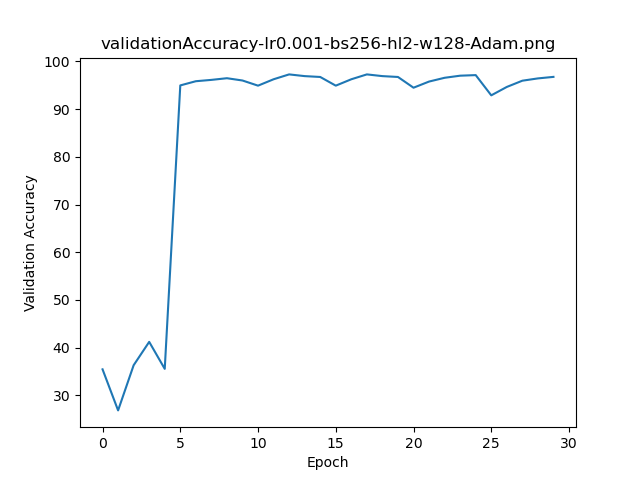
\includegraphics[width=\linewidth]{testsResults/validationAccuracy/validationAccuracy-lr0.001-bs256-hl2-w128-Adam.png}
        \caption{Default settings + batching size = 256}
        \endminipage
    \end{figure}

\subsubsection{Number of Hidden Layers}

    \begin{figure}[H]
        \minipage{0.5\textwidth}
        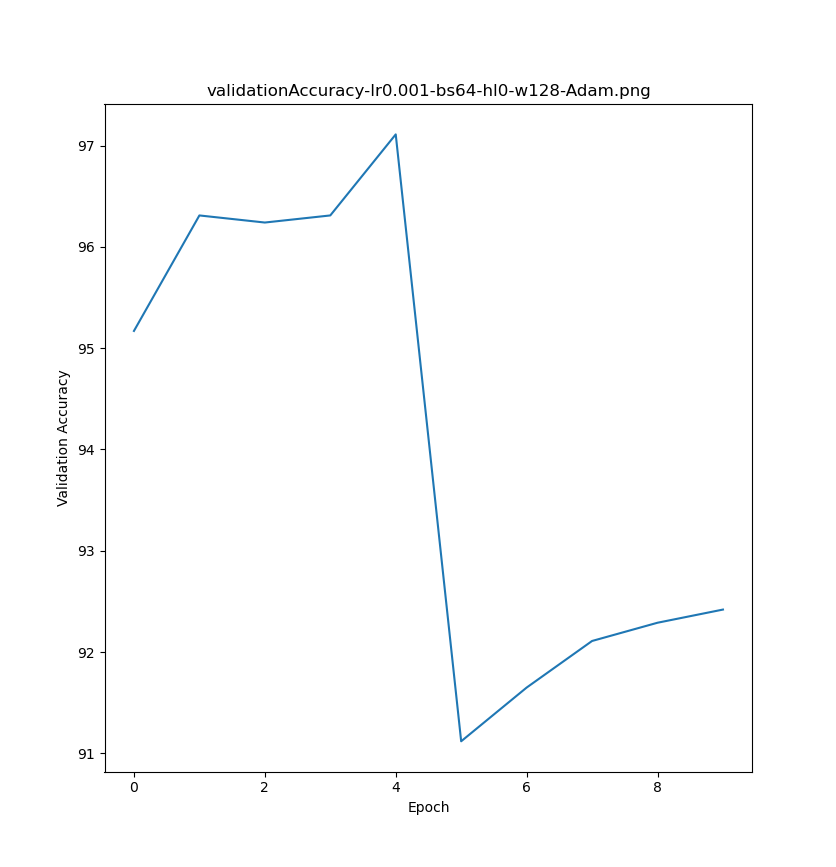
\includegraphics[width=\linewidth]{testsResults/validationAccuracy/validationAccuracyhl0.png}
        \caption{Default settings + hidden layers = 0}
        \endminipage\hfill
        \minipage{0.5\textwidth}
        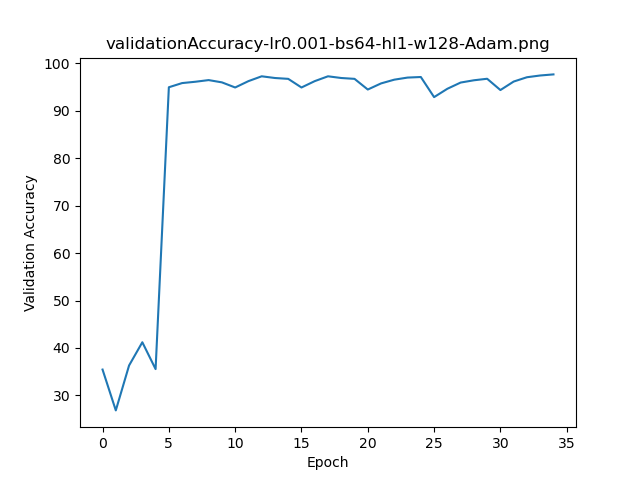
\includegraphics[width=\linewidth]{testsResults/validationAccuracy/validationAccuracy-lr0.001-bs64-hl1-w128-Adam.png}
        \caption{Default settings + hidden layers = 1}
        \endminipage
    \end{figure}
        \begin{figure}[H]
        \minipage{0.5\textwidth}%
        \includegraphics[width=\linewidth]{testsResults/validationAccuracy/def.png}
        \caption{Default settings + hidden layers = 2}
        \endminipage
        \minipage{0.5\textwidth}%
        \includegraphics[width=\linewidth]{testsResults/validationAccuracy/validationAccuracy-lr0.001-bs64-hl3-w128-Adam.png}
        \caption{Default settings + hidden layers = 3}
        \endminipage
    \end{figure}
    \newpage
\subsubsection{Width}

    \begin{figure}[H]
        \minipage{0.5\textwidth}
        \includegraphics[width=\linewidth]{testsResults/validationAccuracy/def.png}
        \caption{Default settings + width = 128}
        \endminipage\hfill
        \minipage{0.5\textwidth}
        \includegraphics[width=\linewidth]{testsResults/validationAccuracy/validationAccuracy-lr0.001-bs64-hl2-w64-Adam.png}
        \caption{Default settings + width = 64}
        \endminipage
    \end{figure}
        \begin{figure}[H]
        \minipage{0.5\textwidth}%
        \includegraphics[width=\linewidth]{testsResults/validationAccuracy/validationAccuracy-lr0.001-bs64-hl2-w256-Adam.png}
        \caption{Default settings + width = 256}
        \endminipage
        \minipage{0.5\textwidth}%
        \includegraphics[width=\linewidth]{testsResults/validationAccuracy/validationAccuracy-lr0.001-bs64-hl2-w512-Adam.png}
        \caption{Default settings + width = 512}
        \endminipage
    \end{figure}
    \begin{figure}[H]
        \minipage{0.5\textwidth}%
        \includegraphics[width=\linewidth]{testsResults/validationAccuracy/validationAccuracy-lr0.001-bs64-hl2-w1024-Adam.png}
        \caption{Default settings + width = 1024}
        \endminipage
    \end{figure}

\subsubsection{Optimizer Type}

    \begin{figure}[H]
        \minipage{0.5\textwidth}
        \includegraphics[width=\linewidth]{testsResults/validationAccuracy/def.png}
        \caption{Default settings + Adam optimizer}
        \endminipage\hfill
        \minipage{0.5\textwidth}
        \includegraphics[width=\linewidth]{testsResults/validationAccuracy/validationAccuracy-lr0.001-bs64-hl2-w128-SGD.png}
        \caption{Default settings + learning rate = 0.01}
        \endminipage
    \end{figure}
        \begin{figure}[H]
        \minipage{0.5\textwidth}%
        \includegraphics[width=\linewidth]{testsResults/validationAccuracy/validationAccuracy-lr0.001-bs64-hl2-w128-SGD_Momentum.png}
        \caption{Default settings + SGD\_Momentum optimizer}
        \endminipage
    \end{figure}

    \subsection{Speed}
    We also checked how different parameters impact speed of the neural network learning 

    \paragraph{Changing learning rate}
    \begin{center}
        \begin{tabular}{ | c | c |  }
            \hline
         Learning rate & Execution Time [s] \\ 
         \hline
         0.001 (default) & 49.3 \\  
         \hline
         0.01 & 53.9 \\    
         \hline
         0.1 & 50.1 \\    
         \hline
    \end{tabular}
    \end{center}

    \paragraph{Changing batch size}
    \begin{center}
        \begin{tabular}{ | c | c |  }
            \hline
         Batch Size & Execution Time [s] \\ 
         \hline
         1 & 567.2 (!) \\  
         \hline
         64 (default) & 49.3 \\    
         \hline
         128 & 48.1 \\    
         \hline
         256 & 42.8 \\    
         \hline
         
    \end{tabular}
    \end{center}

    \paragraph{Changing number of hidden layers}
    \begin{center}
        \begin{tabular}{ | c | c |  }
            \hline
         Hidden layers & Execution Time [s] \\ 
         \hline
         0 & 44.5 \\  
         \hline
         1 & 48.8 \\    
         \hline
         2 (default) & 49.3 \\    
         \hline
         3 & 48.7 \\    
         \hline
    \end{tabular}
    \end{center}

    \paragraph{Changing width}
    \begin{center}
        \begin{tabular}{ | c | c |  }
            \hline
         Width & Execution Time [s] \\ 
         \hline
         64 & 46.7 \\  
         \hline
         128 (default) & 49.3 \\    
         \hline
         256 & 49.0 \\    
         \hline
         512 & 52.1 \\    
         \hline
         1024 & 73.9 \\    
         \hline
    \end{tabular}
    \end{center}

    \paragraph{Changing optimizer type}
    \begin{center}
        \begin{tabular}{ | c | c |  }
            \hline
         Learning rate & Execution Time [s] \\ 
         \hline
         Adam (default) & 49.3 \\  
         \hline
         SGD & 45.1 \\    
         \hline
         SGD Momentum & 45.5 \\    
         \hline
    \end{tabular}
    \end{center}

    \paragraph{Analysis}
    Two parameters that had the biggest impact on execution time was setting batch size to extremely low value (1) and increasing width (jump between 512 width and 1024 is equal to 20 seconds more execution time)

\end{document}
